% Options for packages loaded elsewhere
\PassOptionsToPackage{unicode}{hyperref}
\PassOptionsToPackage{hyphens}{url}
%
\documentclass[
]{article}
\usepackage{amsmath,amssymb}
\usepackage{lmodern}
\usepackage{iftex}
\ifPDFTeX
  \usepackage[T1]{fontenc}
  \usepackage[utf8]{inputenc}
  \usepackage{textcomp} % provide euro and other symbols
\else % if luatex or xetex
  \usepackage{unicode-math}
  \defaultfontfeatures{Scale=MatchLowercase}
  \defaultfontfeatures[\rmfamily]{Ligatures=TeX,Scale=1}
\fi
% Use upquote if available, for straight quotes in verbatim environments
\IfFileExists{upquote.sty}{\usepackage{upquote}}{}
\IfFileExists{microtype.sty}{% use microtype if available
  \usepackage[]{microtype}
  \UseMicrotypeSet[protrusion]{basicmath} % disable protrusion for tt fonts
}{}
\makeatletter
\@ifundefined{KOMAClassName}{% if non-KOMA class
  \IfFileExists{parskip.sty}{%
    \usepackage{parskip}
  }{% else
    \setlength{\parindent}{0pt}
    \setlength{\parskip}{6pt plus 2pt minus 1pt}}
}{% if KOMA class
  \KOMAoptions{parskip=half}}
\makeatother
\usepackage{xcolor}
\IfFileExists{xurl.sty}{\usepackage{xurl}}{} % add URL line breaks if available
\IfFileExists{bookmark.sty}{\usepackage{bookmark}}{\usepackage{hyperref}}
\hypersetup{
  pdftitle={dns\_first},
  hidelinks,
  pdfcreator={LaTeX via pandoc}}
\urlstyle{same} % disable monospaced font for URLs
\usepackage[margin=1in]{geometry}
\usepackage{color}
\usepackage{fancyvrb}
\newcommand{\VerbBar}{|}
\newcommand{\VERB}{\Verb[commandchars=\\\{\}]}
\DefineVerbatimEnvironment{Highlighting}{Verbatim}{commandchars=\\\{\}}
% Add ',fontsize=\small' for more characters per line
\usepackage{framed}
\definecolor{shadecolor}{RGB}{248,248,248}
\newenvironment{Shaded}{\begin{snugshade}}{\end{snugshade}}
\newcommand{\AlertTok}[1]{\textcolor[rgb]{0.94,0.16,0.16}{#1}}
\newcommand{\AnnotationTok}[1]{\textcolor[rgb]{0.56,0.35,0.01}{\textbf{\textit{#1}}}}
\newcommand{\AttributeTok}[1]{\textcolor[rgb]{0.77,0.63,0.00}{#1}}
\newcommand{\BaseNTok}[1]{\textcolor[rgb]{0.00,0.00,0.81}{#1}}
\newcommand{\BuiltInTok}[1]{#1}
\newcommand{\CharTok}[1]{\textcolor[rgb]{0.31,0.60,0.02}{#1}}
\newcommand{\CommentTok}[1]{\textcolor[rgb]{0.56,0.35,0.01}{\textit{#1}}}
\newcommand{\CommentVarTok}[1]{\textcolor[rgb]{0.56,0.35,0.01}{\textbf{\textit{#1}}}}
\newcommand{\ConstantTok}[1]{\textcolor[rgb]{0.00,0.00,0.00}{#1}}
\newcommand{\ControlFlowTok}[1]{\textcolor[rgb]{0.13,0.29,0.53}{\textbf{#1}}}
\newcommand{\DataTypeTok}[1]{\textcolor[rgb]{0.13,0.29,0.53}{#1}}
\newcommand{\DecValTok}[1]{\textcolor[rgb]{0.00,0.00,0.81}{#1}}
\newcommand{\DocumentationTok}[1]{\textcolor[rgb]{0.56,0.35,0.01}{\textbf{\textit{#1}}}}
\newcommand{\ErrorTok}[1]{\textcolor[rgb]{0.64,0.00,0.00}{\textbf{#1}}}
\newcommand{\ExtensionTok}[1]{#1}
\newcommand{\FloatTok}[1]{\textcolor[rgb]{0.00,0.00,0.81}{#1}}
\newcommand{\FunctionTok}[1]{\textcolor[rgb]{0.00,0.00,0.00}{#1}}
\newcommand{\ImportTok}[1]{#1}
\newcommand{\InformationTok}[1]{\textcolor[rgb]{0.56,0.35,0.01}{\textbf{\textit{#1}}}}
\newcommand{\KeywordTok}[1]{\textcolor[rgb]{0.13,0.29,0.53}{\textbf{#1}}}
\newcommand{\NormalTok}[1]{#1}
\newcommand{\OperatorTok}[1]{\textcolor[rgb]{0.81,0.36,0.00}{\textbf{#1}}}
\newcommand{\OtherTok}[1]{\textcolor[rgb]{0.56,0.35,0.01}{#1}}
\newcommand{\PreprocessorTok}[1]{\textcolor[rgb]{0.56,0.35,0.01}{\textit{#1}}}
\newcommand{\RegionMarkerTok}[1]{#1}
\newcommand{\SpecialCharTok}[1]{\textcolor[rgb]{0.00,0.00,0.00}{#1}}
\newcommand{\SpecialStringTok}[1]{\textcolor[rgb]{0.31,0.60,0.02}{#1}}
\newcommand{\StringTok}[1]{\textcolor[rgb]{0.31,0.60,0.02}{#1}}
\newcommand{\VariableTok}[1]{\textcolor[rgb]{0.00,0.00,0.00}{#1}}
\newcommand{\VerbatimStringTok}[1]{\textcolor[rgb]{0.31,0.60,0.02}{#1}}
\newcommand{\WarningTok}[1]{\textcolor[rgb]{0.56,0.35,0.01}{\textbf{\textit{#1}}}}
\usepackage{graphicx}
\makeatletter
\def\maxwidth{\ifdim\Gin@nat@width>\linewidth\linewidth\else\Gin@nat@width\fi}
\def\maxheight{\ifdim\Gin@nat@height>\textheight\textheight\else\Gin@nat@height\fi}
\makeatother
% Scale images if necessary, so that they will not overflow the page
% margins by default, and it is still possible to overwrite the defaults
% using explicit options in \includegraphics[width, height, ...]{}
\setkeys{Gin}{width=\maxwidth,height=\maxheight,keepaspectratio}
% Set default figure placement to htbp
\makeatletter
\def\fps@figure{htbp}
\makeatother
\setlength{\emergencystretch}{3em} % prevent overfull lines
\providecommand{\tightlist}{%
  \setlength{\itemsep}{0pt}\setlength{\parskip}{0pt}}
\setcounter{secnumdepth}{-\maxdimen} % remove section numbering
\ifLuaTeX
  \usepackage{selnolig}  % disable illegal ligatures
\fi

\title{dns\_first}
\author{}
\date{\vspace{-2.5em}2022-03-05}

\begin{document}
\maketitle

\hypertarget{r-markdown}{%
\subsection{R Markdown}\label{r-markdown}}

\begin{Shaded}
\begin{Highlighting}[]
\FunctionTok{library}\NormalTok{(}\StringTok{\textquotesingle{}RSQLite\textquotesingle{}}\NormalTok{)}
\FunctionTok{library}\NormalTok{(}\StringTok{\textquotesingle{}ggplot2\textquotesingle{}}\NormalTok{)}
\FunctionTok{library}\NormalTok{(DBI)}
\FunctionTok{options}\NormalTok{(}\StringTok{"scipen"}\OtherTok{=}\DecValTok{100}\NormalTok{, }\StringTok{"digits"}\OtherTok{=}\DecValTok{4}\NormalTok{)}


\NormalTok{db }\OtherTok{\textless{}{-}} \FunctionTok{dbConnect}\NormalTok{(RSQLite}\SpecialCharTok{::}\FunctionTok{SQLite}\NormalTok{(), }\AttributeTok{dbname=}\StringTok{"./dnstor\_statistics\_dns.sqlite"}\NormalTok{)}
\NormalTok{dns\_data }\OtherTok{\textless{}{-}}\FunctionTok{dbSendQuery}\NormalTok{(db, }\StringTok{"  }
\StringTok{  SELECT count(*) as countGrouped, year, period, CAST(CAST(year AS text) || CAST(period AS text) as integer) as year\_period , qname, qtype, SUM(count) as quantity}
\StringTok{    FROM DNS\_ANALYSIS}
\StringTok{GROUP BY year\_period, year, period, qname, qtype}
\StringTok{ORDER BY quantity DESC;}
\StringTok{"}\NormalTok{)}
\NormalTok{dns\_data\_fetched }\OtherTok{\textless{}{-}} \FunctionTok{fetch}\NormalTok{(dns\_data)}
\CommentTok{\#dns\_data\_fetched}

\CommentTok{\#str(dns\_data\_fetched)}
\CommentTok{\#str(dns\_data\_fetched$payload)}
\end{Highlighting}
\end{Shaded}

\begin{Shaded}
\begin{Highlighting}[]
\FunctionTok{library}\NormalTok{(dplyr)}
\end{Highlighting}
\end{Shaded}

\begin{verbatim}
## 
## Attaching package: 'dplyr'
\end{verbatim}

\begin{verbatim}
## The following objects are masked from 'package:stats':
## 
##     filter, lag
\end{verbatim}

\begin{verbatim}
## The following objects are masked from 'package:base':
## 
##     intersect, setdiff, setequal, union
\end{verbatim}

\begin{Shaded}
\begin{Highlighting}[]
\FunctionTok{library}\NormalTok{(tibble)}

\NormalTok{dns\_data.year\_period.ungrouped }\OtherTok{\textless{}{-}} \FunctionTok{group\_split}\NormalTok{(dns\_data\_fetched, year\_period) }

\NormalTok{N }\OtherTok{=} \DecValTok{10}
\NormalTok{dns\_data.topNconsultas }\OtherTok{\textless{}{-}} \FunctionTok{head}\NormalTok{(dns\_data.year\_period.ungrouped[[}\DecValTok{1}\NormalTok{]], N)}
\NormalTok{dns\_data.year\_period.ungrouped.len }\OtherTok{=} \FunctionTok{length}\NormalTok{(dns\_data.year\_period.ungrouped)}

\ControlFlowTok{for}\NormalTok{ (i }\ControlFlowTok{in} \FunctionTok{c}\NormalTok{(}\DecValTok{2}\SpecialCharTok{:}\NormalTok{dns\_data.year\_period.ungrouped.len)) \{}
\NormalTok{  dns\_data.topNconsultas }\OtherTok{\textless{}{-}} \FunctionTok{rbind}\NormalTok{(dns\_data.topNconsultas, }\FunctionTok{head}\NormalTok{(dns\_data.year\_period.ungrouped[[i]], N))}
\NormalTok{\}}

\CommentTok{\#dns\_data.year\_period.ungrouped[[1]]}
\CommentTok{\#ggplot(dns\_data.year\_period.ungrouped[[1]], aes(x=qname, y=quantity), ) + geom\_histogram(fill="skyblue", alpha=0.5) }
\CommentTok{\#ggplot(data = dns\_data.year\_period.ungrouped[[1]], aes(x = qname, y = quantity)) +}
 \CommentTok{\#geom\_boxplot()}

\CommentTok{\#dns\_data.topNconsultas}

\CommentTok{\#dns\_data.year\_period.ungrouped}

\CommentTok{\#dns\_data\_fetched[order(dns\_data\_fetched$year, dns\_data\_fetched$period, {-}dns\_data\_fetched$quantity),]}

\CommentTok{\#dns\_data\_fetched}

\CommentTok{\# ggplot(request, aes(x=rt, fill=Type)) + geom\_density(alpha=0.4) + scale\_x\_log10() + xlab("Number Request (log 10)") + ylab("Density") + ggtitle("Request per DRDoS Attacks")}
\CommentTok{\# barplot}
\CommentTok{\#  ggplot(nlme::Oxboys, aes(age, height))}

\CommentTok{\# Top N consultas por período N = 10}
\FunctionTok{head}\NormalTok{(dns\_data.topNconsultas)}
\end{Highlighting}
\end{Shaded}

\begin{verbatim}
## # A tibble: 6 x 7
##   countGrouped  year period year_period qname           qtype quantity
##          <int> <int>  <int>       <int> <chr>           <chr>    <int>
## 1        23891  2020      4       20204 peacecorps.gov. ANY   19005578
## 2        49615  2020      4       20204 lavrov.in.      ANY     816242
## 3          777  2020      4       20204 sl.             ANY     779892
## 4        45508  2020      4       20204 irs.gov.        ANY     652325
## 5         1336  2020      4       20204 fe18.ru.        ANY     569411
## 6          354  2020      4       20204 .               ANY      12296
\end{verbatim}

\begin{Shaded}
\begin{Highlighting}[]
\FunctionTok{ggplot}\NormalTok{(dns\_data\_fetched, }\FunctionTok{aes}\NormalTok{(}\AttributeTok{x=}\NormalTok{year\_period), ) }\SpecialCharTok{+} \FunctionTok{geom\_histogram}\NormalTok{(}\AttributeTok{fill=}\StringTok{"skyblue"}\NormalTok{, }\AttributeTok{alpha=}\FloatTok{0.5}\NormalTok{) }
\end{Highlighting}
\end{Shaded}

\begin{verbatim}
## `stat_bin()` using `bins = 30`. Pick better value with `binwidth`.
\end{verbatim}

\includegraphics{dns_first_files/figure-latex/unnamed-chunk-2-1.pdf}

\begin{Shaded}
\begin{Highlighting}[]
\FunctionTok{ggplot}\NormalTok{(dns\_data.topNconsultas, }\FunctionTok{aes}\NormalTok{(qname,quantity, }\AttributeTok{group =} \DecValTok{1}\NormalTok{)) }\SpecialCharTok{+} \FunctionTok{geom\_line}\NormalTok{() }\SpecialCharTok{+} \FunctionTok{facet\_grid}\NormalTok{(year\_period }\SpecialCharTok{\textasciitilde{}}\NormalTok{ .)}
\end{Highlighting}
\end{Shaded}

\includegraphics{dns_first_files/figure-latex/unnamed-chunk-2-2.pdf}

\begin{Shaded}
\begin{Highlighting}[]
\CommentTok{\#ggplot(data = dns\_data.topNconsultas) + }
 \CommentTok{\# geom\_point(mapping = aes(x = year\_period, y = quantity)) + }
  \CommentTok{\#facet\_wrap(\textasciitilde{} class, nrow = 2)}

\CommentTok{\#ggplot(data = dns\_data.topNconsultas) + }
 \CommentTok{\# geom\_bar(mapping = aes(x = year\_period, y = count, fill = year\_period), position = "fill")}


\DocumentationTok{\#\# {-}{-}{-}{-}{-}{-}{-}{-}{-}{-}{-}{-} Quantos ataques com cada tipo de qtype foi utilizado, por trimestre ? {-}{-}{-}{-}{-}{-}{-}{-}{-}{-}{-}{-}}
\CommentTok{\#dns\_data\_fetched}

\NormalTok{dns\_data\_fetched.quarter\_type\_quantity }\OtherTok{=} \FunctionTok{select}\NormalTok{(dns\_data\_fetched, }\FunctionTok{c}\NormalTok{(}\StringTok{\textquotesingle{}year\_period\textquotesingle{}}\NormalTok{, }\StringTok{\textquotesingle{}qtype\textquotesingle{}}\NormalTok{, }\StringTok{\textquotesingle{}quantity\textquotesingle{}}\NormalTok{))}

\CommentTok{\#dns\_data\_fetched.quarter\_type\_quantity}
\CommentTok{\#typeof(dns\_data\_fetched$year\_period)}
\CommentTok{\#dns\_data\_fetched$year\_period}

\CommentTok{\#dns\_data\_fetched.quarter\_type\_quantity[order(dns\_data\_fetched.quarter\_type\_quantity$year\_period),]}

\NormalTok{dns\_data\_fetched.sum\_attacks\_quarterly }\OtherTok{=}\NormalTok{ dns\_data\_fetched.quarter\_type\_quantity }\SpecialCharTok{\%\textgreater{}\%}
  \FunctionTok{group\_by}\NormalTok{(qtype, year\_period) }\SpecialCharTok{\%\textgreater{}\%}
  \FunctionTok{summarise}\NormalTok{(}\AttributeTok{quantity =} \FunctionTok{sum}\NormalTok{(quantity))}
\end{Highlighting}
\end{Shaded}

\begin{verbatim}
## `summarise()` has grouped output by 'qtype'. You can override using the
## `.groups` argument.
\end{verbatim}

\begin{Shaded}
\begin{Highlighting}[]
\CommentTok{\#dns\_data\_fetched.sum\_attacks\_quarterly[order({-}dns\_data\_fetched.sum\_attacks\_quarterly$quantity, dns\_data\_fetched.sum\_attacks\_quarterly$year\_period),]}

\FunctionTok{ggplot}\NormalTok{(}\AttributeTok{data =}\NormalTok{ dns\_data\_fetched.sum\_attacks\_quarterly, }\FunctionTok{aes}\NormalTok{(}\AttributeTok{x =}\NormalTok{ year\_period, }\AttributeTok{y =}\NormalTok{ quantity, }\AttributeTok{color =}\NormalTok{ qtype)) }\SpecialCharTok{+}
    \FunctionTok{geom\_line}\NormalTok{()}
\end{Highlighting}
\end{Shaded}

\includegraphics{dns_first_files/figure-latex/unnamed-chunk-2-3.pdf}

\begin{Shaded}
\begin{Highlighting}[]
\FunctionTok{ggplot}\NormalTok{(}\AttributeTok{data =}\NormalTok{ dns\_data\_fetched.sum\_attacks\_quarterly, }\FunctionTok{aes}\NormalTok{(}\AttributeTok{x =}\NormalTok{ year\_period, }\AttributeTok{y =}\NormalTok{ quantity)) }\SpecialCharTok{+}
    \FunctionTok{geom\_line}\NormalTok{() }\SpecialCharTok{+}
    \FunctionTok{facet\_wrap}\NormalTok{(}\AttributeTok{facets =} \FunctionTok{vars}\NormalTok{(qtype))}
\end{Highlighting}
\end{Shaded}

\begin{verbatim}
## geom_path: Each group consists of only one observation. Do you need to adjust
## the group aesthetic?
\end{verbatim}

\begin{verbatim}
## geom_path: Each group consists of only one observation. Do you need to adjust
## the group aesthetic?
\end{verbatim}

\includegraphics{dns_first_files/figure-latex/unnamed-chunk-2-4.pdf}

\begin{Shaded}
\begin{Highlighting}[]
\CommentTok{\#aggregate(x = dns\_data\_fetched.quarter\_type\_quantity, FUN = "sum", drop = TRUE)}

\CommentTok{\# {-}{-}{-}{-}{-}{-}{-}{-}{-}{-}{-}{-} Quantos qtypes novos aprecem em cada trimestre {-}{-}{-}{-}{-}{-}{-}{-}{-}{-}{-}{-}}
\CommentTok{\# \textgreater{} Diferenças percentuais são mais relevantes que absolutas}

\NormalTok{quarter\_qtype\_aux }\OtherTok{=}\NormalTok{ dns\_data.year\_period.ungrouped[[}\DecValTok{1}\NormalTok{]] }\SpecialCharTok{\%\textgreater{}\%}
  \FunctionTok{group\_by}\NormalTok{(qtype) }\SpecialCharTok{\%\textgreater{}\%}
  \FunctionTok{summarise}\NormalTok{(}\AttributeTok{quantity =} \FunctionTok{sum}\NormalTok{(quantity))}

\CommentTok{\#quarter\_qtype\_2 = dns\_data.year\_period.ungrouped[[2]] \%\textgreater{}\%}
\CommentTok{\#  group\_by(qtype) \%\textgreater{}\%}
\CommentTok{\#  summarise(quantity = sum(quantity))}

\CommentTok{\#quarter\_qtype\_2}
\CommentTok{\#merged = merge(x = quarter\_qtype\_aux, y = quarter\_qtype\_2, by = "qtype", all = TRUE)}
\CommentTok{\#merged.new\_quantity = merged$quantity.x {-} merged$quantity.y}
\CommentTok{\#merged}




\NormalTok{quarter\_new\_qtype }\OtherTok{=} \FunctionTok{data.frame}\NormalTok{()}



\ControlFlowTok{for}\NormalTok{ (i }\ControlFlowTok{in} \FunctionTok{c}\NormalTok{(}\DecValTok{2}\SpecialCharTok{:}\NormalTok{dns\_data.year\_period.ungrouped.len)) \{}
\NormalTok{  quarter\_qtype }\OtherTok{=}\NormalTok{ dns\_data.year\_period.ungrouped[[i]] }\SpecialCharTok{\%\textgreater{}\%}
    \FunctionTok{group\_by}\NormalTok{(qtype) }\SpecialCharTok{\%\textgreater{}\%}
    \FunctionTok{summarise}\NormalTok{(}\AttributeTok{quantity =} \FunctionTok{sum}\NormalTok{(quantity))}
  
\NormalTok{  merged }\OtherTok{=} \FunctionTok{merge}\NormalTok{(}\AttributeTok{x =}\NormalTok{ quarter\_qtype\_aux, }\AttributeTok{y =}\NormalTok{ quarter\_qtype, }\AttributeTok{by =} \StringTok{"qtype"}\NormalTok{, }\AttributeTok{all =} \ConstantTok{TRUE}\NormalTok{)}
\NormalTok{  merged.new\_quantity }\OtherTok{=}\NormalTok{ merged}\SpecialCharTok{$}\NormalTok{quantity.x }\SpecialCharTok{{-}}\NormalTok{ merged}\SpecialCharTok{$}\NormalTok{quantity.y}
  
\NormalTok{  perio\_to\_period }\OtherTok{=} \FunctionTok{paste}\NormalTok{(}\FunctionTok{head}\NormalTok{(dns\_data.year\_period.ungrouped[[i }\SpecialCharTok{{-}} \DecValTok{1}\NormalTok{]][}\StringTok{\textquotesingle{}year\textquotesingle{}}\NormalTok{], }\DecValTok{1}\NormalTok{), }\StringTok{\textquotesingle{}.\textquotesingle{}}\NormalTok{,  }\FunctionTok{head}\NormalTok{(dns\_data.year\_period.ungrouped[[i }\SpecialCharTok{{-}} \DecValTok{1}\NormalTok{]][}\StringTok{\textquotesingle{}period\textquotesingle{}}\NormalTok{], }\DecValTok{1}\NormalTok{), }\StringTok{\textquotesingle{}{-}\textgreater{}\textquotesingle{}}\NormalTok{ , }\FunctionTok{head}\NormalTok{(dns\_data.year\_period.ungrouped[[i]][}\StringTok{\textquotesingle{}year\textquotesingle{}}\NormalTok{], }\DecValTok{1}\NormalTok{), }\StringTok{\textquotesingle{}.\textquotesingle{}}\NormalTok{, }\FunctionTok{head}\NormalTok{(dns\_data.year\_period.ungrouped[[i]][}\StringTok{\textquotesingle{}period\textquotesingle{}}\NormalTok{], }\DecValTok{1}\NormalTok{))}
\NormalTok{  quarter\_new\_qtype }\OtherTok{\textless{}{-}} \FunctionTok{rbind}\NormalTok{(quarter\_new\_qtype, }\FunctionTok{data.frame}\NormalTok{(}\AttributeTok{quarter\_to\_quarter=}\NormalTok{perio\_to\_period, merged}\SpecialCharTok{$}\NormalTok{qtype, }\AttributeTok{sum\_quantity=}\NormalTok{merged}\SpecialCharTok{$}\NormalTok{quantity.y }\SpecialCharTok{{-}}\NormalTok{ merged}\SpecialCharTok{$}\NormalTok{quantity.x, }\AttributeTok{quantity\_percentage=}\NormalTok{(((merged}\SpecialCharTok{$}\NormalTok{quantity.y }\SpecialCharTok{{-}}\NormalTok{ merged}\SpecialCharTok{$}\NormalTok{quantity.x)}\SpecialCharTok{*}\DecValTok{100}\NormalTok{)}\SpecialCharTok{/}\NormalTok{merged}\SpecialCharTok{$}\NormalTok{quantity.x), merged}\SpecialCharTok{$}\NormalTok{quantity.x, merged}\SpecialCharTok{$}\NormalTok{quantity.y))}
  
\NormalTok{  quarter\_qtype\_aux }\OtherTok{=}\NormalTok{ quarter\_qtype}
\NormalTok{\}}

\CommentTok{\#quarter\_new\_qtype}
\FunctionTok{head}\NormalTok{(}\FunctionTok{na.omit}\NormalTok{(quarter\_new\_qtype[}\FunctionTok{order}\NormalTok{(}\SpecialCharTok{{-}}\NormalTok{quarter\_new\_qtype}\SpecialCharTok{$}\NormalTok{quantity\_percentage),]))}
\end{Highlighting}
\end{Shaded}

\begin{verbatim}
##      quarter_to_quarter merged.qtype sum_quantity quantity_percentage
## 30 2021 . 2 -> 2021 . 3        RRSIG       325120             26803.0
## 18 2021 . 1 -> 2021 . 2           NS          119              2975.0
## 35 2021 . 3 -> 2021 . 4          ANY      5133467              1480.4
## 24 2021 . 2 -> 2021 . 3         AAAA          195               367.9
## 6  2020 . 4 -> 2021 . 1           MX       111066               336.9
## 46 2021 . 4 -> 2022 . 1           NS            2               200.0
##    merged.quantity.x merged.quantity.y
## 30              1213            326333
## 18                 4               123
## 35            346754           5480221
## 24                53               248
## 6              32964            144030
## 46                 1                 3
\end{verbatim}

\begin{Shaded}
\begin{Highlighting}[]
\CommentTok{\# {-}{-}{-}{-}{-}{-}{-}{-}{-}{-}{-}{-} Quantos qname novos aprecem em cada trimestre {-}{-}{-}{-}{-}{-}{-}{-}{-}{-}{-}{-}}

\NormalTok{quarter\_qname\_aux }\OtherTok{=}\NormalTok{ dns\_data.year\_period.ungrouped[[}\DecValTok{1}\NormalTok{]] }\SpecialCharTok{\%\textgreater{}\%}
  \FunctionTok{group\_by}\NormalTok{(qname) }\SpecialCharTok{\%\textgreater{}\%}
  \FunctionTok{summarise}\NormalTok{(}\AttributeTok{quantity =} \FunctionTok{sum}\NormalTok{(quantity))}

\NormalTok{quarter\_new\_qname }\OtherTok{=} \FunctionTok{data.frame}\NormalTok{()}
\ControlFlowTok{for}\NormalTok{ (i }\ControlFlowTok{in} \FunctionTok{c}\NormalTok{(}\DecValTok{2}\SpecialCharTok{:}\NormalTok{dns\_data.year\_period.ungrouped.len)) \{}
\NormalTok{  quarter\_qname }\OtherTok{=}\NormalTok{ dns\_data.year\_period.ungrouped[[i]] }\SpecialCharTok{\%\textgreater{}\%}
    \FunctionTok{group\_by}\NormalTok{(qname) }\SpecialCharTok{\%\textgreater{}\%}
    \FunctionTok{summarise}\NormalTok{(}\AttributeTok{quantity =} \FunctionTok{sum}\NormalTok{(quantity))}
  
\NormalTok{  merged }\OtherTok{=} \FunctionTok{merge}\NormalTok{(}\AttributeTok{x =}\NormalTok{ quarter\_qname\_aux, }\AttributeTok{y =}\NormalTok{ quarter\_qname, }\AttributeTok{by =} \StringTok{"qname"}\NormalTok{, }\AttributeTok{all =} \ConstantTok{TRUE}\NormalTok{)}
\NormalTok{  merged.new\_quantity }\OtherTok{=}\NormalTok{ merged}\SpecialCharTok{$}\NormalTok{quantity.x }\SpecialCharTok{{-}}\NormalTok{ merged}\SpecialCharTok{$}\NormalTok{quantity.y}
  
\NormalTok{  period\_to\_period }\OtherTok{=} \FunctionTok{paste}\NormalTok{(}\FunctionTok{head}\NormalTok{(dns\_data.year\_period.ungrouped[[i }\SpecialCharTok{{-}} \DecValTok{1}\NormalTok{]][}\StringTok{\textquotesingle{}year\textquotesingle{}}\NormalTok{], }\DecValTok{1}\NormalTok{), }\StringTok{\textquotesingle{}.\textquotesingle{}}\NormalTok{,  }\FunctionTok{head}\NormalTok{(dns\_data.year\_period.ungrouped[[i }\SpecialCharTok{{-}} \DecValTok{1}\NormalTok{]][}\StringTok{\textquotesingle{}period\textquotesingle{}}\NormalTok{], }\DecValTok{1}\NormalTok{), }\StringTok{\textquotesingle{}{-}\textgreater{}\textquotesingle{}}\NormalTok{ , }\AttributeTok{... =} \FunctionTok{head}\NormalTok{(dns\_data.year\_period.ungrouped[[i]][}\StringTok{\textquotesingle{}year\textquotesingle{}}\NormalTok{], }\DecValTok{1}\NormalTok{), }\StringTok{\textquotesingle{}.\textquotesingle{}}\NormalTok{, }\FunctionTok{head}\NormalTok{(dns\_data.year\_period.ungrouped[[i]][}\StringTok{\textquotesingle{}period\textquotesingle{}}\NormalTok{], }\DecValTok{1}\NormalTok{))}
\NormalTok{  quarter\_new\_qname }\OtherTok{\textless{}{-}} \FunctionTok{rbind}\NormalTok{(quarter\_new\_qname, }\FunctionTok{data.frame}\NormalTok{(}\AttributeTok{quarter\_to\_quarter=}\NormalTok{period\_to\_period, merged}\SpecialCharTok{$}\NormalTok{qname, }\AttributeTok{sum\_quantity=}\NormalTok{(merged}\SpecialCharTok{$}\NormalTok{quantity.y }\SpecialCharTok{{-}}\NormalTok{ merged}\SpecialCharTok{$}\NormalTok{quantity.x), }\AttributeTok{quantity\_percentage\_diff=}\NormalTok{(((merged}\SpecialCharTok{$}\NormalTok{quantity.y }\SpecialCharTok{{-}}\NormalTok{ merged}\SpecialCharTok{$}\NormalTok{quantity.x)}\SpecialCharTok{*}\DecValTok{100}\NormalTok{)}\SpecialCharTok{/}\NormalTok{merged}\SpecialCharTok{$}\NormalTok{quantity.x), merged}\SpecialCharTok{$}\NormalTok{quantity.x, merged}\SpecialCharTok{$}\NormalTok{quantity.y))}
  
\NormalTok{  quarter\_qname\_aux }\OtherTok{=}\NormalTok{ quarter\_qname}
\NormalTok{\}}
\CommentTok{\#quarter\_new\_qname}
\FunctionTok{head}\NormalTok{(}\FunctionTok{na.omit}\NormalTok{(quarter\_new\_qname[}\SpecialCharTok{{-}}\FunctionTok{order}\NormalTok{(quarter\_new\_qname}\SpecialCharTok{$}\NormalTok{quantity\_percentage\_diff),]))}
\end{Highlighting}
\end{Shaded}

\begin{verbatim}
## [1] quarter_to_quarter       merged.qname             sum_quantity            
## [4] quantity_percentage_diff merged.quantity.x        merged.quantity.y       
## <0 rows> (or 0-length row.names)
\end{verbatim}

\begin{Shaded}
\begin{Highlighting}[]
\CommentTok{\#1{-} olhar a longo prazo, o timelapse dos qnames}
\CommentTok{\#2{-} qual a frequencia d qnames novos nesses períodos}
 \CommentTok{\#   2.1 olhar em detalhes as variações dos qnames (pq geralmente eles acabam sendo um grupo)}
\end{Highlighting}
\end{Shaded}

\begin{Shaded}
\begin{Highlighting}[]
\CommentTok{\# Vale um gráfico de barras (dois, um agrupado e outro empilhado) da porcentagem de QTYPEs por período}
\CommentTok{\# https://www.data{-}to{-}viz.com/graph/barplot.html}
\CommentTok{\# Libraries}
\CommentTok{\#library(tidyverse)}
\CommentTok{\#library(hrbrthemes)}
\FunctionTok{library}\NormalTok{(viridis)}
\end{Highlighting}
\end{Shaded}

\begin{verbatim}
## Loading required package: viridisLite
\end{verbatim}

\begin{Shaded}
\begin{Highlighting}[]
\NormalTok{dns\_data\_fetched.sum\_attacks\_quarterly.quantity\_percentage }\OtherTok{=}\NormalTok{ dns\_data\_fetched.sum\_attacks\_quarterly}\SpecialCharTok{$}\NormalTok{quantity }\SpecialCharTok{/} \DecValTok{2}
\CommentTok{\#dns\_data\_fetched.sum\_attacks\_quarterly}

\NormalTok{dns\_data\_fetched.sum\_attacks\_quarterly.sum\_period }\OtherTok{=}\NormalTok{ dns\_data\_fetched.sum\_attacks\_quarterly }\SpecialCharTok{\%\textgreater{}\%}
  \FunctionTok{group\_by}\NormalTok{(year\_period) }\SpecialCharTok{\%\textgreater{}\%}
  \FunctionTok{summarise}\NormalTok{(}\AttributeTok{period\_quantity =} \FunctionTok{sum}\NormalTok{(quantity), }\AttributeTok{qtype=}\NormalTok{qtype, }\AttributeTok{quantity=}\NormalTok{quantity)}
\end{Highlighting}
\end{Shaded}

\begin{verbatim}
## `summarise()` has grouped output by 'year_period'. You can override using the
## `.groups` argument.
\end{verbatim}

\begin{Shaded}
\begin{Highlighting}[]
\NormalTok{dns\_data\_fetched.sum\_attacks\_quarterly.sum\_period[}\StringTok{\textquotesingle{}quantity\_percentage\textquotesingle{}}\NormalTok{] }\OtherTok{=}\NormalTok{ (dns\_data\_fetched.sum\_attacks\_quarterly.sum\_period}\SpecialCharTok{$}\NormalTok{quantity }\SpecialCharTok{*} \DecValTok{100}\NormalTok{) }\SpecialCharTok{/}\NormalTok{ dns\_data\_fetched.sum\_attacks\_quarterly.sum\_period}\SpecialCharTok{$}\NormalTok{period\_quantity}

\CommentTok{\#dns\_data\_fetched.sum\_attacks\_quarterly.sum\_period}


\NormalTok{dns\_data\_fetched.sum\_attacks\_quarterly.sum\_period }\SpecialCharTok{\%\textgreater{}\%} 
  \FunctionTok{mutate}\NormalTok{(}\AttributeTok{year\_period=}\FunctionTok{as.factor}\NormalTok{(year\_period)) }\SpecialCharTok{\%\textgreater{}\%}
  \FunctionTok{ggplot}\NormalTok{( }\FunctionTok{aes}\NormalTok{(}\AttributeTok{x=}\NormalTok{year\_period, }\AttributeTok{y=}\NormalTok{quantity\_percentage, }\AttributeTok{fill=}\NormalTok{qtype)) }\SpecialCharTok{+}
    \FunctionTok{geom\_bar}\NormalTok{(}\AttributeTok{stat=}\StringTok{"identity"}\NormalTok{, }\AttributeTok{position=}\StringTok{"dodge"}\NormalTok{) }\SpecialCharTok{+}
    \FunctionTok{scale\_fill\_viridis}\NormalTok{(}\AttributeTok{discrete=}\ConstantTok{TRUE}\NormalTok{, }\AttributeTok{name=}\StringTok{""}\NormalTok{) }\SpecialCharTok{+}
    \FunctionTok{ylab}\NormalTok{(}\StringTok{"Percentage of attacks"}\NormalTok{) }\SpecialCharTok{+}
    \FunctionTok{ggtitle}\NormalTok{(}\StringTok{"All QTYPES {-} ungrouped bar"}\NormalTok{)}
\end{Highlighting}
\end{Shaded}

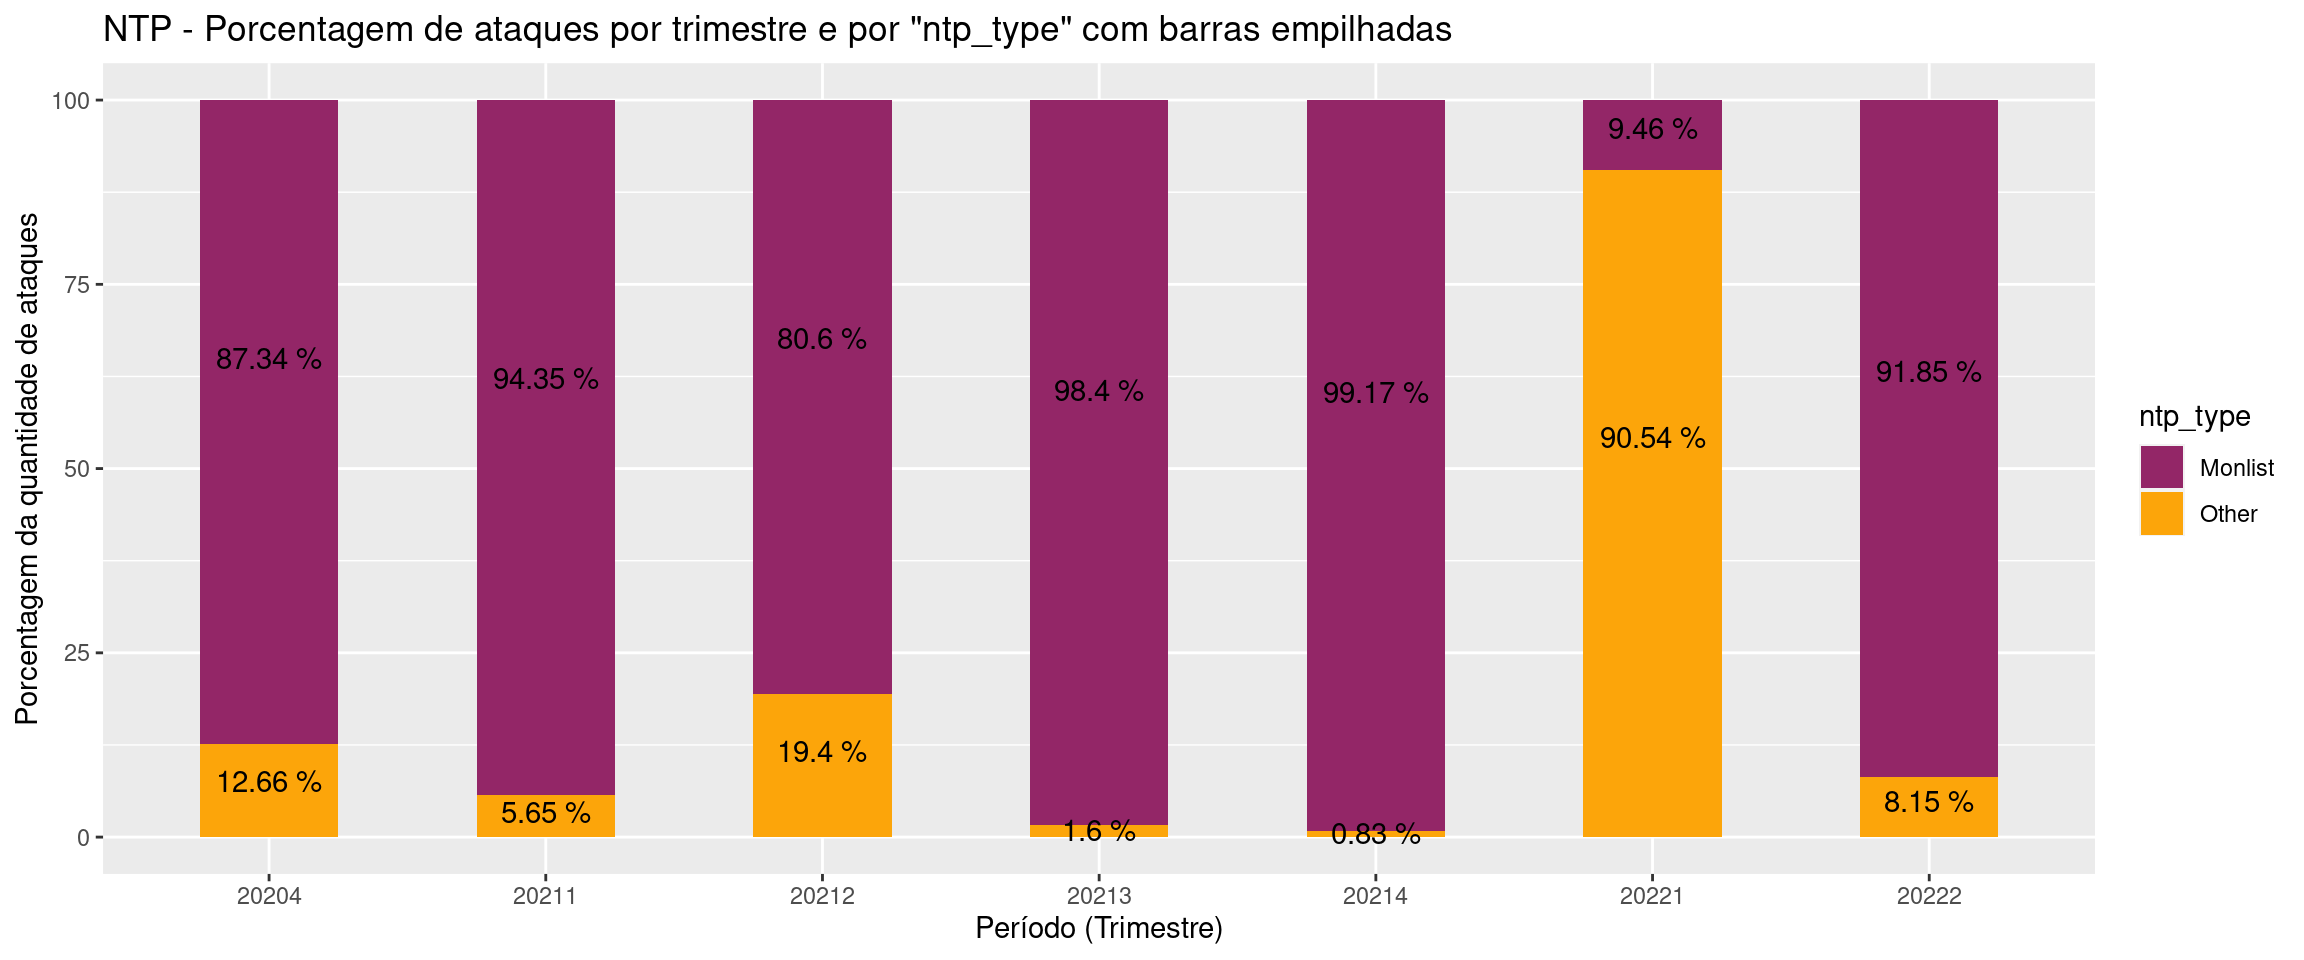
\includegraphics{dns_first_files/figure-latex/unnamed-chunk-3-1.pdf}

\begin{Shaded}
\begin{Highlighting}[]
\NormalTok{dns\_data\_fetched.sum\_attacks\_quarterly.sum\_period }\SpecialCharTok{\%\textgreater{}\%} 
  \FunctionTok{mutate}\NormalTok{(}\AttributeTok{year\_period=}\FunctionTok{as.factor}\NormalTok{(year\_period)) }\SpecialCharTok{\%\textgreater{}\%}
  \FunctionTok{ggplot}\NormalTok{( }\FunctionTok{aes}\NormalTok{(}\AttributeTok{x=}\NormalTok{year\_period, }\AttributeTok{y=}\NormalTok{quantity\_percentage, }\AttributeTok{fill=}\NormalTok{qtype)) }\SpecialCharTok{+}
    \FunctionTok{geom\_bar}\NormalTok{(}\AttributeTok{stat=}\StringTok{"identity"}\NormalTok{, }\AttributeTok{width =} \FloatTok{0.5}\NormalTok{) }\SpecialCharTok{+}
    \FunctionTok{scale\_fill\_viridis}\NormalTok{(}\AttributeTok{discrete=}\ConstantTok{TRUE}\NormalTok{, }\AttributeTok{name=}\StringTok{""}\NormalTok{) }\SpecialCharTok{+}
    \FunctionTok{ylab}\NormalTok{(}\StringTok{"Percentage of attacks"}\NormalTok{) }\SpecialCharTok{+}
    \FunctionTok{ggtitle}\NormalTok{(}\StringTok{"All QTYPES {-} stacked bars"}\NormalTok{)}
\end{Highlighting}
\end{Shaded}

\includegraphics{dns_first_files/figure-latex/unnamed-chunk-3-2.pdf}

\begin{Shaded}
\begin{Highlighting}[]
\DocumentationTok{\#\# Filter data using qtype quantity percentage bigger than 1}

\NormalTok{dns\_data\_fetched.sum\_attacks\_quarterly.sum\_period }\SpecialCharTok{\%\textgreater{}\%}
  \FunctionTok{filter}\NormalTok{(quantity\_percentage }\SpecialCharTok{\textgreater{}} \DecValTok{1}\NormalTok{) }\SpecialCharTok{\%\textgreater{}\%}
  \FunctionTok{mutate}\NormalTok{(}\AttributeTok{year\_period=}\FunctionTok{as.factor}\NormalTok{(year\_period)) }\SpecialCharTok{\%\textgreater{}\%}
  \FunctionTok{ggplot}\NormalTok{( }\FunctionTok{aes}\NormalTok{(}\AttributeTok{x=}\NormalTok{year\_period, }\AttributeTok{y=}\NormalTok{quantity\_percentage, }\AttributeTok{fill=}\NormalTok{qtype)) }\SpecialCharTok{+}
    \FunctionTok{geom\_bar}\NormalTok{(}\AttributeTok{stat=}\StringTok{"identity"}\NormalTok{, }\AttributeTok{position=}\StringTok{"dodge"}\NormalTok{) }\SpecialCharTok{+}
    \FunctionTok{scale\_fill\_viridis}\NormalTok{(}\AttributeTok{discrete=}\ConstantTok{TRUE}\NormalTok{, }\AttributeTok{name=}\StringTok{""}\NormalTok{) }\SpecialCharTok{+}
    \FunctionTok{ylab}\NormalTok{(}\StringTok{"Percentage of attacks"}\NormalTok{) }\SpecialCharTok{+}
    \FunctionTok{ggtitle}\NormalTok{(}\StringTok{"QTYPES \textgreater{} 1\% by period {-} ungrouped bars"}\NormalTok{)}
\end{Highlighting}
\end{Shaded}

\includegraphics{dns_first_files/figure-latex/unnamed-chunk-3-3.pdf}

\begin{Shaded}
\begin{Highlighting}[]
\NormalTok{dns\_data\_fetched.sum\_attacks\_quarterly.sum\_period }\SpecialCharTok{\%\textgreater{}\%}
  \FunctionTok{filter}\NormalTok{(quantity\_percentage }\SpecialCharTok{\textgreater{}} \DecValTok{1}\NormalTok{) }\SpecialCharTok{\%\textgreater{}\%}
  \FunctionTok{mutate}\NormalTok{(}\AttributeTok{year\_period=}\FunctionTok{as.factor}\NormalTok{(year\_period)) }\SpecialCharTok{\%\textgreater{}\%}
  \FunctionTok{ggplot}\NormalTok{( }\FunctionTok{aes}\NormalTok{(}\AttributeTok{x=}\NormalTok{year\_period, }\AttributeTok{y=}\NormalTok{quantity\_percentage, }\AttributeTok{fill=}\NormalTok{qtype)) }\SpecialCharTok{+}
    \FunctionTok{geom\_bar}\NormalTok{(}\AttributeTok{stat=}\StringTok{"identity"}\NormalTok{, }\AttributeTok{width =} \FloatTok{0.5}\NormalTok{) }\SpecialCharTok{+}
    \FunctionTok{scale\_fill\_viridis}\NormalTok{(}\AttributeTok{discrete=}\ConstantTok{TRUE}\NormalTok{, }\AttributeTok{name=}\StringTok{""}\NormalTok{) }\SpecialCharTok{+}
    \FunctionTok{ylab}\NormalTok{(}\StringTok{"Percentage of attacks"}\NormalTok{) }\SpecialCharTok{+}
    \FunctionTok{ggtitle}\NormalTok{(}\StringTok{"QTYPES \textgreater{} 1\% by period {-} stacked bars"}\NormalTok{)}
\end{Highlighting}
\end{Shaded}

\includegraphics{dns_first_files/figure-latex/unnamed-chunk-3-4.pdf}

\begin{Shaded}
\begin{Highlighting}[]
\CommentTok{\#dns\_data\_fetched.sum\_attacks\_quarterly.sum\_period}
\NormalTok{dns\_data\_fetched.sum\_attacks\_quarterly.sum\_period.relevant }\OtherTok{=}\NormalTok{ dns\_data\_fetched.sum\_attacks\_quarterly.sum\_period }\SpecialCharTok{\%\textgreater{}\%} 
  \FunctionTok{filter}\NormalTok{(quantity\_percentage }\SpecialCharTok{\textgreater{}} \DecValTok{1}\NormalTok{)}

\CommentTok{\#dns\_data\_fetched.sum\_attacks\_quarterly.sum\_period.relevant$qtype}
\NormalTok{qtypes\_bigger\_1 }\OtherTok{=}\NormalTok{ dns\_data\_fetched.sum\_attacks\_quarterly.sum\_period.relevant}\SpecialCharTok{$}\NormalTok{qtype[}\SpecialCharTok{!}\FunctionTok{duplicated}\NormalTok{(dns\_data\_fetched.sum\_attacks\_quarterly.sum\_period.relevant}\SpecialCharTok{$}\NormalTok{qtype)]}
\CommentTok{\#qtypes\_bigger\_1}

\NormalTok{dns\_data\_fetched.sum\_attacks\_quarterly.sum\_period }\SpecialCharTok{\%\textgreater{}\%}
  \FunctionTok{filter}\NormalTok{(qtype }\SpecialCharTok{\%in\%}\NormalTok{ qtypes\_bigger\_1) }\SpecialCharTok{\%\textgreater{}\%}
  \FunctionTok{mutate}\NormalTok{(}\AttributeTok{year\_period=}\FunctionTok{as.factor}\NormalTok{(year\_period)) }\SpecialCharTok{\%\textgreater{}\%}
  \FunctionTok{ggplot}\NormalTok{( }\FunctionTok{aes}\NormalTok{(}\AttributeTok{x=}\NormalTok{year\_period, }\AttributeTok{y=}\NormalTok{quantity\_percentage, }\AttributeTok{fill=}\NormalTok{qtype)) }\SpecialCharTok{+}
    \FunctionTok{geom\_bar}\NormalTok{(}\AttributeTok{stat=}\StringTok{"identity"}\NormalTok{, }\AttributeTok{position=}\StringTok{"dodge"}\NormalTok{) }\SpecialCharTok{+}
    \FunctionTok{scale\_fill\_viridis}\NormalTok{(}\AttributeTok{discrete=}\ConstantTok{TRUE}\NormalTok{, }\AttributeTok{name=}\StringTok{""}\NormalTok{) }\SpecialCharTok{+}
    \FunctionTok{ylab}\NormalTok{(}\StringTok{"Percentage of attacks"}\NormalTok{) }\SpecialCharTok{+}
    \FunctionTok{ggtitle}\NormalTok{(}\StringTok{"Any QTYPE \textgreater{} 1\% {-} ungrouped bars"}\NormalTok{)}
\end{Highlighting}
\end{Shaded}

\includegraphics{dns_first_files/figure-latex/unnamed-chunk-3-5.pdf}

\begin{Shaded}
\begin{Highlighting}[]
\NormalTok{dns\_data\_fetched.sum\_attacks\_quarterly.sum\_period }\SpecialCharTok{\%\textgreater{}\%}
  \FunctionTok{filter}\NormalTok{(qtype }\SpecialCharTok{\%in\%}\NormalTok{ qtypes\_bigger\_1) }\SpecialCharTok{\%\textgreater{}\%}
  \FunctionTok{mutate}\NormalTok{(}\AttributeTok{year\_period=}\FunctionTok{as.factor}\NormalTok{(year\_period)) }\SpecialCharTok{\%\textgreater{}\%}
  \FunctionTok{ggplot}\NormalTok{( }\FunctionTok{aes}\NormalTok{(}\AttributeTok{x=}\NormalTok{year\_period, }\AttributeTok{y=}\NormalTok{quantity\_percentage, }\AttributeTok{fill=}\NormalTok{qtype)) }\SpecialCharTok{+}
    \FunctionTok{geom\_bar}\NormalTok{(}\AttributeTok{stat=}\StringTok{"identity"}\NormalTok{, }\AttributeTok{width =} \FloatTok{0.5}\NormalTok{) }\SpecialCharTok{+}
    \FunctionTok{scale\_fill\_viridis}\NormalTok{(}\AttributeTok{discrete=}\ConstantTok{TRUE}\NormalTok{, }\AttributeTok{name=}\StringTok{""}\NormalTok{) }\SpecialCharTok{+}
    \FunctionTok{ylab}\NormalTok{(}\StringTok{"Percentage of attacks"}\NormalTok{) }\SpecialCharTok{+}
    \FunctionTok{ggtitle}\NormalTok{(}\StringTok{"Any QTYPE \textgreater{} 1\% {-} stacked bars"}\NormalTok{)}
\end{Highlighting}
\end{Shaded}

\includegraphics{dns_first_files/figure-latex/unnamed-chunk-3-6.pdf}

\end{document}
